\documentclass{article}
\usepackage{graphicx}
\usepackage{listings}
\def\lstxml{
  \lstset{language=XML,
    keywordstyle=\ttfamily,
    identifierstyle=\ttfamily,
    stringstyle=\ttfamily,
    showstringspaces=false,
    columns=[l]flexible,
    escapeinside={(@*}{*@)},
    morekeywords={encoding,
      mrow,math,mfrac,mi,msqrt,mo,mn,span,nobr,img}
  }
}

\def\lstjs{
  \lstset{language=Java,
    keywordstyle=\ttfamily,
    identifierstyle=\ttfamily\bfseries, 
    stringstyle=\ttfamily,
    showstringspaces=false,
    columns=[l]flexible, 
    morekeywords={cvox,Api,Math,defineRule}
  }
}
\setlength{\parindent}{0cm}
\pagestyle{empty}

\begin{document}

\section*{Fraction Example}

\textbf{Mathematics:}
\[ \frac{numerator}{denominator} \]

\textbf{MathML representation:}
\lstxml
\begin{lstlisting}
<mfrac>
  <mrow>Numerator</mrow>
  <mrow>Denominator</mrow>
</mfrac>
\end{lstlisting}

\textbf{JavaScript rule:}
\lstjs
\begin{lstlisting}
  defineRule(
      'mfrac', 'default.short', 
          '[t] "Start Frac";
           [n] ./*[1]; 
           [t] "Over";
           [n] ./*[2]; 
           [t] "End Frac"',
      'self::mathml:mfrac');
\end{lstlisting}

\textbf{GUI Mock:}\vspace*{1ex}

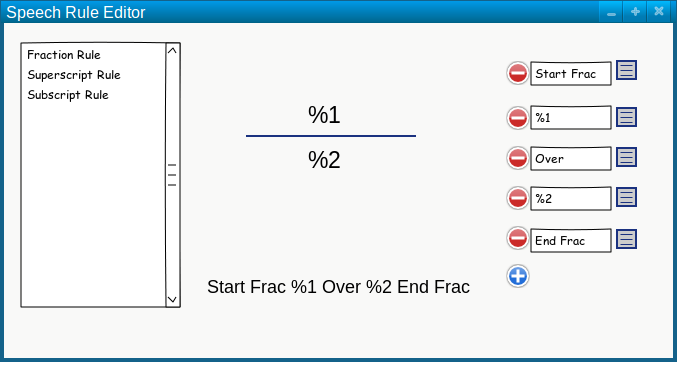
\includegraphics[width=\linewidth]{Editor_Mock}

\end{document}

%%% Local Variables:
%%% mode: latex
%%% TeX-master: t
%%% End:
